\section{Weka}
\label{sect:weka}
One of the most popular ways of drawing insights from data through machine
learning is by using a predefined library.  This is because the library takes
much of the technical effort out of the development.  All of the math behind the
machine learning is hidden behind the library and often there are nice user
interfaces or APIs associated with the library.  Typically, there are many
different methods that can be called to comb throught the data to extract
insights and relationships about the data.  In the case of ProGENitor the Weka
library was chosen as it has an excellent Java API and access to many different
methods.  Choosing the method to extract information from the data requires some
knowledge about the data itself.  In this case, clustering was chosen as the
data is mostly nominal data and the goal is to define some grouping that leads
to the end goal.  To extract the data, first the ProGENitor has to generate an
Arrf file to feed into Weka and then Weka has to evaluate it with the clustering
classification.

\subsection{Arff Creation}
Weka uses the .arrf file format to feed data into the weka toolset.  The Arrf
file contains two major sections.  These sections are the header section and the
data section.\cite{arrf}  The header contains the name of the relation, a list
of attributes, and their types.  The data section, contains the data that will
be used for machine learning.  A sample .arff file would look like the
following:
\\*
\\*
@relation education\\*
\\*
@attribute degree {PHD,Bachelors,Masters}\\*
@attribute
specialization{Electrical,Circuits,Analog,ComputerArchitecture,Digital}\\*
@attribute goal {true,false}\\*
\\*
@data\\*
Bachelors,Electrical,false\\*
Masters,Circuits,false\\*
Bachelors,Electrical,true\\*
Masters,Circuits,true\\*
PHD,MSU,Digital,true\\*

ProGENitor currently generates the .arff file containing just the educational
nodes.  One of the keys to getting quality insights out of Weka is controlling
the data being fed into the tools.  Thus, in this case only the educational data
is fed into the tool.  This process could easily be replicated for additional
insights.  To generate the arff file, ProGENitor contains a Java method called
generate arff in the connections package.  This code follows the procedure
detailed in figure \ref{fig:arrf generation} to generate the arff file that is
later used by Weka.

\usetikzlibrary{shapes,arrows,chains}

\begin{figure}[H]
	\centering
% Start the picture
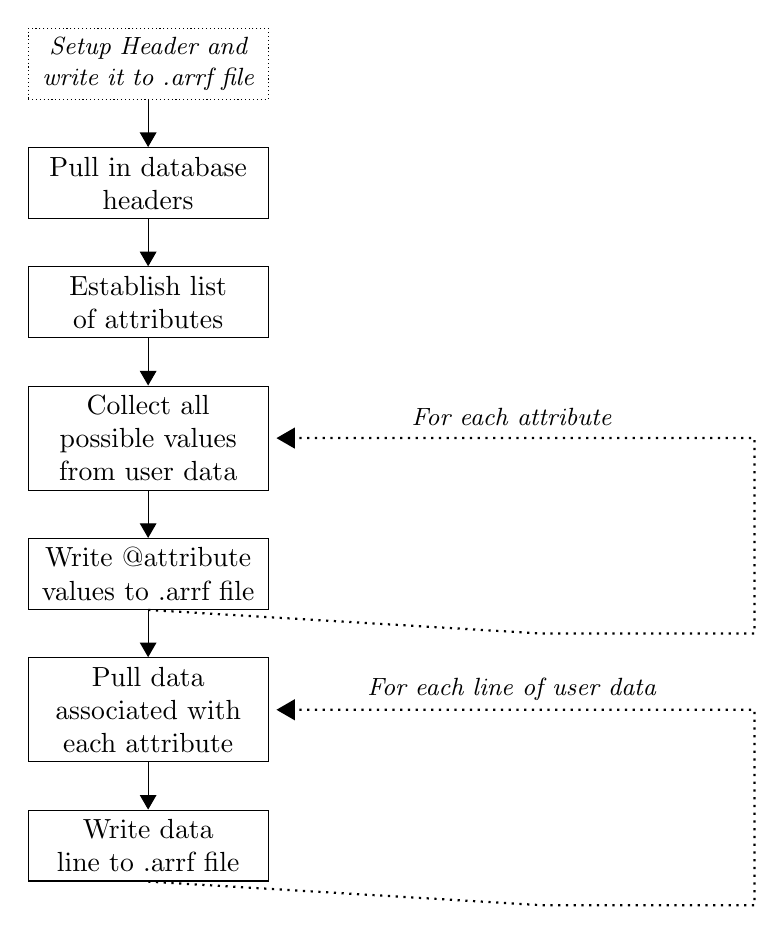
\begin{tikzpicture}[%
    >=triangle 60,              % Nice arrows; your taste may be different
    start chain=going below,    % General flow is top-to-bottom
    node distance=6mm and 60mm, % Global setup of box spacing
    every join/.style={norm},   % Default linetype for connecting boxes
    ]
% ------------------------------------------------- 
% A few box styles 
% <on chain> *and* <on grid> reduce the need for manual relative
% positioning of nodes
\tikzset{
  base/.style={draw, on chain, on grid, align=center, minimum height=4ex},
  proc/.style={base, rectangle, text width=8em},
  test/.style={base, diamond, aspect=2, text width=5em},
  % Connector line styles for different parts of the diagram
  norm/.style={->, draw},
  it/.style={font={\small\itshape}}
}
% -------------------------------------------------
% Start by placing the nodes
\node [proc, densely dotted, it] (p0) {Setup Header and write it to .arrf file};
% Use join to connect a node to the previous one 
\node [proc, join] (p1) {Pull in database headers};
\node [proc, join] (p2) {Establish list of attributes};
\node [proc, join] (p3) {Collect all possible values from user data};
\node [proc, join] (p4) {Write @attribute values to .arrf file}; 
\node [proc, join] (p5) {Pull data associated with each attribute};
\node [proc, join] (p6) {Write data line to .arrf file};

\draw [->, dotted, thick, shorten >=1mm]
  (p4.south) -- ++(50mm,-3mm)  -- ++(27mm,0) 
  |- node [black, near end, yshift=0.75em, it]
    {For each attribute} (p3);

\draw [->, dotted, thick, shorten >=1mm]
  (p6.south) -- ++(50mm,-3mm)  -- ++(27mm,0) 
  |- node [black, near end, yshift=0.75em, it]
    {For each line of user data} (p5);

% -------------------------------------------------
\end{tikzpicture}
	\caption{Arrf File Generation}
	\label{fig:arrf generation}
\end{figure}

\subsection{Clustering}
One major advantage to using the Weka library is it takes complex code and makes
it relatively simple.  As seen in Figure \ref{fig:clustering}, the process that is
followed to analyze the data in the Arrf file is very simple and straight
forward.  Once the Weka jar is imported into the project, the code is very quick
to implement as good documentation is available for the API.\cite{weka}  The
complex portion of work is then ensuring that the appropriate classification is
used and then parsing the data to be returned in a useful fashion.


\usetikzlibrary{shapes,arrows,chains}

\begin{figure}[H]
	\centering
% Start the picture
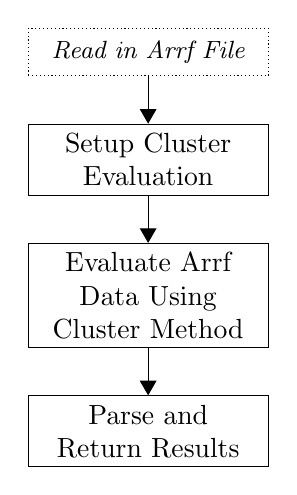
\begin{tikzpicture}[%
    >=triangle 60,              % Nice arrows; your taste may be different
    start chain=going below,    % General flow is top-to-bottom
    node distance=6mm and 60mm, % Global setup of box spacing
    every join/.style={norm},   % Default linetype for connecting boxes
    ]
% ------------------------------------------------- 
% A few box styles 
% <on chain> *and* <on grid> reduce the need for manual relative
% positioning of nodes
\tikzset{
  base/.style={draw, on chain, on grid, align=center, minimum height=4ex},
  proc/.style={base, rectangle, text width=8em},
  test/.style={base, diamond, aspect=2, text width=5em},
  % Connector line styles for different parts of the diagram
  norm/.style={->, draw},
  it/.style={font={\small\itshape}}
}
% -------------------------------------------------
% Start by placing the nodes
\node [proc, densely dotted, it] (p0) {Read in Arrf File};
% Use join to connect a node to the previous one 
\node [proc, join] (p1) {Setup Cluster Evaluation};
\node [proc, join] (p2) {Evaluate Arrf Data Using Cluster Method};
\node [proc, join] (p3) {Parse and Return Results};
% -------------------------------------------------
\end{tikzpicture}
	\caption{Data Clustering}
	\label{fig:clustering}
\end{figure}
